

\section{Experimental Setup}

\subsection{Evaluation Platforms} We evaluate our approach on and NVIDIA RTX 2080Ti GPU, which integrates 4350 CUDA cores for floating
point computation  and 4350 CUDA core for integer operations. The GPU has a 96KB L1 cache and shared memory. The host machine has a 2.30GHz
Intel Xeon E5-2697 CPU with 252GB memory, running Linux kernel v4.15.0. We use CUDA Toolkit version 10.2.


\subsection{Competing Methods} We compare our approach against the following state-of-the-art image and convolution libraries:
\begin{itemize}
  \item \textbf{cuDNN version 7.6.4}. cuDNN is a state-of-the-art convolution implementation that supports 2D and depth-wise convolutions
      on GPU. Moreover, cuDNN can execute GEMM-, FFT- and Winograd-based convolutions.
  \item \textbf{ArrayFire \cite{Yalamanchili2015}, version 3.6.4}. ArrayFire is a popular image and signal processing library. This
      library implements 2D convolutions on GPU. ArrayFire uses Just In Time compiling for standard arithmetic operations. Thus, the
      first run of an ArrayFire application takes longer than the second run. In the experiment, we run ArrayFire twice in each test and
      record the second runtime.
  \item N\textbf{VIDIA Performance Primitives (NPP)}. This is an image and signal processing library. We use NPP for 2D convolutions
      only.
  \item \textbf{GEMM-im2col (im2col)}. We extract the implementation of the im2col from Caffe \cite{jia2014caffe} and take it as a
      baseline for the 2D and multi-channel 2D convolutions.
  \item Direct implementation of depth-wise convolution. We implement a direct depth-wise convolution without using the proposed reuse algorithms. We take this implementation as a baseline for depth-wise convolution.

\end{itemize}

\subsection{Use Cases}
We apply our approach to three representative convolution operations, single-channel 2D convolution, depth-wise convolution and
multi-channel 2D convolution, described as follows.

\mypara{Single-channel 2D convolution.} This applies a single-channel 2D filter to convolve the input in both horizontal and vertical
directions in a 2D spatial domain. This is a classical and a widely used 2D convolution implementation.

\mypara{Depth-wise convolution.} This applies a bank of single-channel 2D filters to convolve with one multi-channel 2D input, e.g., an
image of three colour channels, R, G and B. We apply a 2D convolution filter to each of the input channel. This technique has been widely
used in embedded CNNs, including MobileNetv2 \cite{Sandler_2018_CVPR}, EfficientNet \cite{tan2019efficientnet} and ShuffleNetv2
\cite{Ma_2018_ECCV}.

\mypara{Multi-channel 2D convolution.} This applies a bank of multi-channel 2D filters convolve with one multi-channel 2D input. The 2D
convolution is performed between one filter channel and the corresponding input channel, and the results are sum up across channels to
generate one output channel.


\subsection{Performance Report} We run each test case ten times on an unloaded machine and report the averaged running time. We found
little variance during execution runs, less than 2\%.  The data type is 32-bit (single-precision) floating point, and all the data are
organized as 4D tensors $(N,C,H,$ and $W)$. In this work, we test 2D, multi-channel 2D and depth-wise convolutions with two filters sizes,
$3 \times 3$ and $5 \times 5$, because these are commonly used filter sizes.
%
%\subsection{Notations}
%Throughout the evaluation, we use $I$, $F$, and $O$ to represent the input, the filter, and the output respectively, $N$, $C$, $H$, and $W$
%to denote the batch size, the channel, the height, and the width, respectively.

\section{Experimental Results}
\label{exp} In this section, we report our results 2D convolution (Section \ref{sec:ex2dc}), depth-wise convolution (Section
\ref{sec:depconvexp}) and multi-channel 2D convolution (Section \ref {multicconvexp}), showing that our approach consistently outperforms
alternative methods for all use cases.


\subsection{Single-Channel 2D Convolution\label{sec:ex2dc}}
\begin{figure*}
\centering
\subfloat[Speedups for the filter of size $3 \times 3$.]{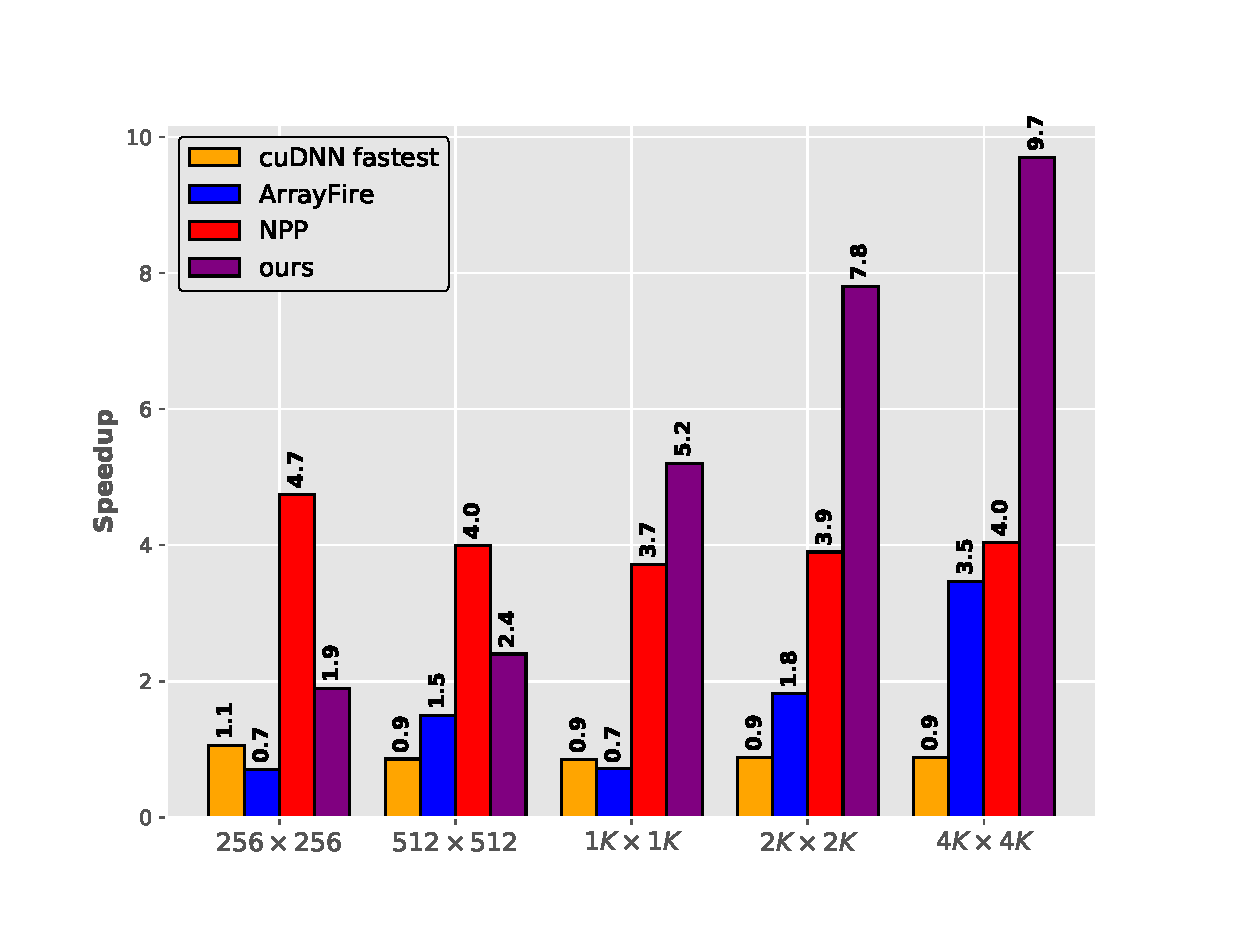
\includegraphics[width=\columnwidth,height=6cm]{./figure/2d_conv_f3.eps}
	\label{fig:2druntimef3c12080}}
\hspace{0em}
\subfloat[Speedups for the filter of size $5 \times 5$.]{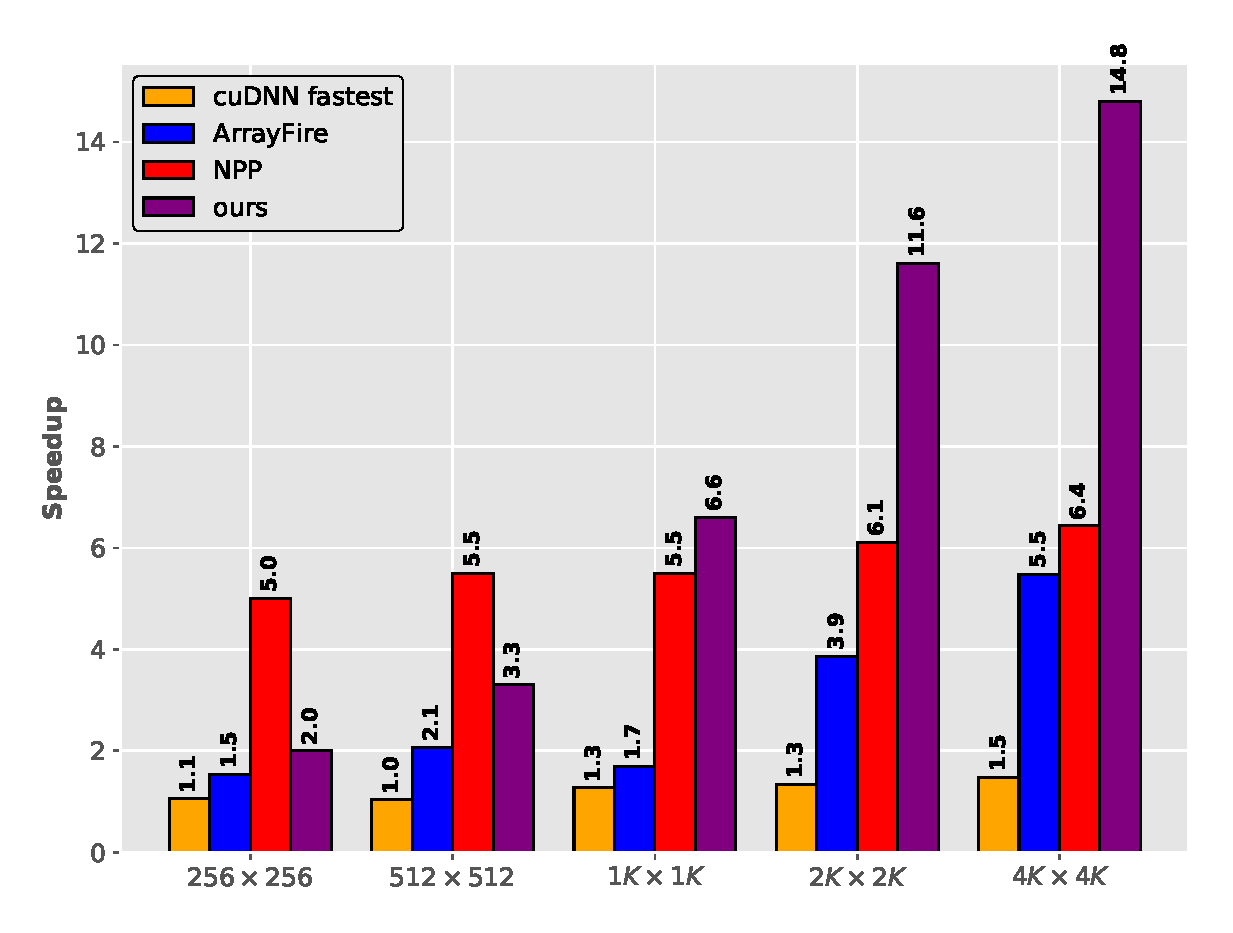
\includegraphics[width=\columnwidth,height=6cm]{./figure/2d_conv_f5.eps}
	\label{fig:2druntimef5c12080}}
	
\caption{Speedups of 2D convolutions of four implementations over im2col.}
\label{fig:2druntime}
\end{figure*}


\subsubsection{Setup}
In this experiment, we compare our approach against the single-channel 2D convolution implementation from cuDNN, GEMM-im2col, ArrayFire,
and NPP. As cuDNN provides multiple implementations, we empirically choose the fastest version, denoted as cuDNN-fastest, for evaluation.
We apply each method to images with sizes ranging from $256 \times 256$ to $4K \times 4K$. We set the batch size, channel, height, and
width of the input to be 1.


\subsubsection{Overall results}
 Figure
\ref{fig:2druntime} reports the speedups of cuDNN, ArrayFire, NPP and our approach over GEMM-im2col. While cuDNN has been heavily optimized
for NVIDIA GPUs, it does not show a notable performance advantage. When using a $3 \times 3$ filter, o ur approach gives the best overall
speedup of 6.5x (up to 9.7x for the largest input), which translates to an improvement of  more than 30\% over the second-best method, NPP.
We note that our approach is based on the standard 2D direct convolution by applying the column and row reuse algorithms. Therefore, the
performance gain is mainly attributed to the reduction of the number of memory transactions. When using a $5 \times 5$ filter, our approach
achieves a better overall speedup of $7.7\times$. A $5 \times 5$ filter has four overlapped columns and rows (instead of just one
overlapped column and row on width and height dimensions when using a $3 \times 3$ filter). The larger number of overlapped data thus give
more room for performance optimization when using our column and row reuse algorithms. Our approach achieves the best overall performance
and demonstrates significant performance advantages when processing large input.

\subsubsection{Further analysis}
\begin{figure}[t!]
\centering

\subfloat[Memory throughput]{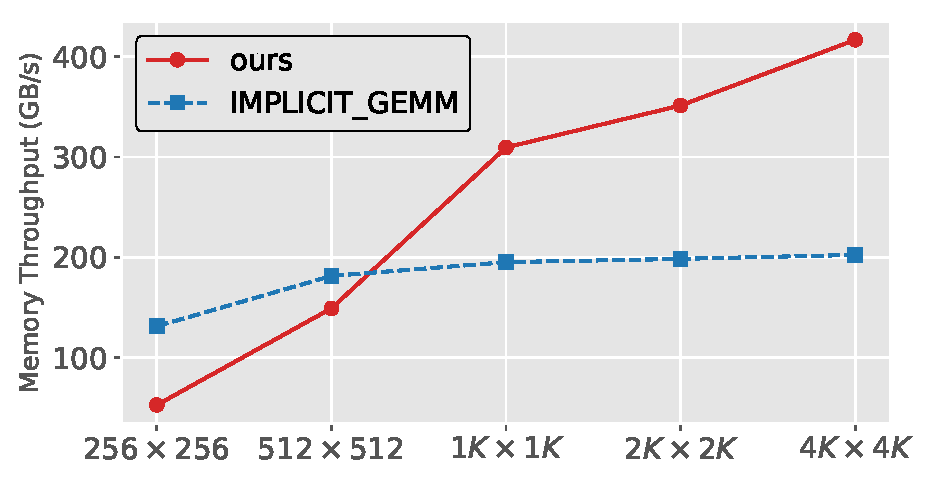
\includegraphics[width=\columnwidth,height=6cm]{./figure/2dmemthroughput.eps}
	\label{fig:2dmemthr}} \hspace{0em}

\subfloat[Maximum bandwidth]{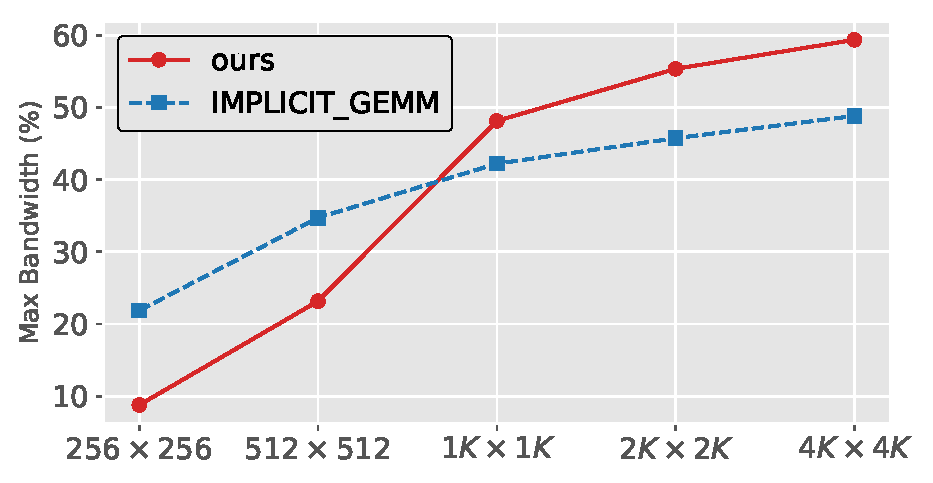
\includegraphics[width=\columnwidth,height=6cm]{./figure/2dmembandwidth.eps}
	\label{fig:2dmaxband}}
	
\caption{Memory profiling of NPP and our approach when applying  a filter of size $3 \times 3$ to single-channel 2D convolution.}
\label{fig:2dmemanaly}
\end{figure}

On the test cases of small input sizes (i.e., $256 \times 256$ and $512 \times 512$), NPP gives the best performance. To understand the
performance gap on small input sizes, we use \emph{nvidia compute} to collect memory profiles, including memory throughput and max
bandwidth, of our implementation and NPP when using a $3 \times 3$ filter to perform convolution. The profiling results are shown in Figure
\ref{fig:2dmemanaly}.  We see that as the input size increases, the memory throughput and the maximum bandwidth also grow. This is expected
as the larger the input image, the larger number the memory transactions is likely to be when performing convolution.  We also observe that
our approach leads to higher memory throughput and the maximum bandwidth used when the input image size is greater or equal than $1K \times
1K$. This finding matches the results presented in Figure \ref{fig:2druntime}, where our approach gives the best performance when
processing an image whose size is $1K \times 1K$ or larger. This result also suggests that memory performance has a strong correlation with
the performance of 2D convolutions.


The reason why our approach gives lower memory throughput and achieves lower maximum bandwidth on small input sizes over NPP is explained
as follows. For single-channel 2D convolution, only one filter is used to convolve with one single-channel input feature map, which
requires much less computation compared to, e.g., the depth-wise or multi-channel convolutions. Therefore, memory performance has a huge
impact on the performance of 2D convolutions. Our row reuse algorithm performs better when a thread operates on more rows of output.
However, the more rows a thread compute on, the fewer warps and thread blocks we can generate. Without enough warps issuing memory
requests, the memory throughput and maximum bandwidth will reduce significantly, which leads to slower performance over NPP. As the input
size increases, we can allocate more thread blocks and more warps per thread block. With enough memory requests and reduction on redundant
memory transactions, we can increase the memory throughput and max bandwidth to improve the performance of 2D convolution.



%Our approach achieves the best speedups in six out of ten test cases. NPP achieves the best results on small image sizes, whereas our
%implementation demonstrates the best results on large image sizes. We use \emph{nvidia compute} to collect memory profiles, including
%memory throughput and max bandwidth, of our implementation and NPP when convolving with a $3 \times 3$ filter. The results are shown in
%Figure \ref{fig:2dmemanaly}.
%
%We can see that as the input size increases, memory throughput and max bandwidth of our implementation exceeds that of NPP, the turning point ($1K \times 1K$ in Figure \ref{fig:2dmemanaly}) is the same as that of speedups in Figure \ref{fig:2druntimef3c12080}, which means that memory performance has a strong relationship with the performance of 2D convolutions. Next, we give a detailed analysis of why the memory throughput and max bandwidth of our implementation is low for small input sizes.
%
%When performing 2D convolutions, only one filter is used to convolve with one single-channel input feature map, which requires much less computation than depth-wise convolutions. Therefore, the memory performance has a huge impact on the performance of 2D convolutions. The proposed row reuse algorithm performs better when a thread calculates more rows of output. However, the more rows each thread calculates, the less warps and thread blocks we can generate. Without enough warps issuing memory requests, the memory throughput and max bandwidth can reduce a lot, which can slow down our implementations. As the input size increases, we can allocate more thread blocks and more warps per thread block. With enough memory requests and reduction on redundant memory transactions, we can increase the memory throughput and max bandwidth, and thus improve the performance of our implementation.
%
%The average speedup of our implementation for $5 \times 5$ filter is $7.7\times$, which is better than the speedup of $5.4\times$ for $3 \times 3$ filter. The key reason for the improvement is that, for $3 \times 3$ filter, there is only one overlapped column and row on width and height dimensions. While for $5 \times 5$ filter, there are four overlapped columns and rows, therefore column and row reuse algorithms can be used more efficiently compared with  that for the $3 \times 3$ filter.





\subsubsection{Summary} Overall, our optimization algorithms can greatly reduce the number of memory transactions and improve the performance of 2D
convolutions. Compared with state-of-the-art image processing libraries, NPP, our approach achieves average speedups of 1.3$\times$ and
1.28$\times$ when using a $3 \times 3$ and $5 \times 5$ filters, respectively.

\subsection{Depth-wise Convolution}
\label{sec:depconvexp}

\begin{table}[]
\caption{Layer configurations of multi-channel 2D convolutions$^{\dag}$.}
\label{tab:3dconvconfigs}
\centering
\rowcolors{2}{}{Gray}
\begin{threeparttable}
\begin{tabular}{lrrrrr}
\toprule
& \textbf{$I_N$} & \textbf{$I_C$} & \textbf{$I_H \times I_W$ }&  \textbf{$F_H \times F_W$} \\
\midrule
\textbf{CONV1} & 512  & 32    & 112*112 & $3 \times 3$, $5 \times 5$  \\
\textbf{CONV2} & 512  & 96    & 112*112  &$3 \times 3$, $5 \times 5$   \\
\textbf{CONV3} & 512  & 144   & 56*56  &$3 \times 3$, $5 \times 5$    \\
\textbf{CONV4} & 512  & 160    & 56*56  &$3 \times 3$, $5 \times 5$    \\
\textbf{CONV5} & 512  & 192   & 28*28  &$3 \times 3$, $5 \times 5$    \\
\textbf{CONV6} & 512  & 240   & 28*28  &$3 \times 3$, $5 \times 5$    \\
\textbf{CONV7} & 512  & 256   & 28*28  &$3 \times 3$, $5 \times 5$    \\
\textbf{CONV8} & 512  & 384   & 14*14  &$3 \times 3$, $5 \times 5$    \\
\textbf{CONV9} & 512  & 480   & 14*14  &$3 \times 3$, $5 \times 5$    \\
\textbf{CONV10} & 512  & 672  & 14*14 &$3 \times 3$, $5 \times 5$     \\
\textbf{CONV11} & 512  &672  & 7*7 & $3 \times 3$, $5 \times 5$      \\
\textbf{CONV12} & 512  &960  & 7*7 & $3 \times 3$, $5 \times 5$      \\
\textbf{CONV13} & 512  &1152  & 7*7 & $3 \times 3$, $5 \times 5$      \\
\bottomrule
\end{tabular}
\footnotesize
\begin{tablenotes}
\item[\dag] We use $I$, $F$, and $O$ to represent the input, the filter, and the output respectively, $N$, $C$, $H$, and $W$
to denote the batch size, the channel, the height, and the width, respectively.
\end{tablenotes}
\end{threeparttable}
\end{table}

\begin{figure*}
\centering
	
\subfloat[Speedups for the filter of size $3 \times 3$.]{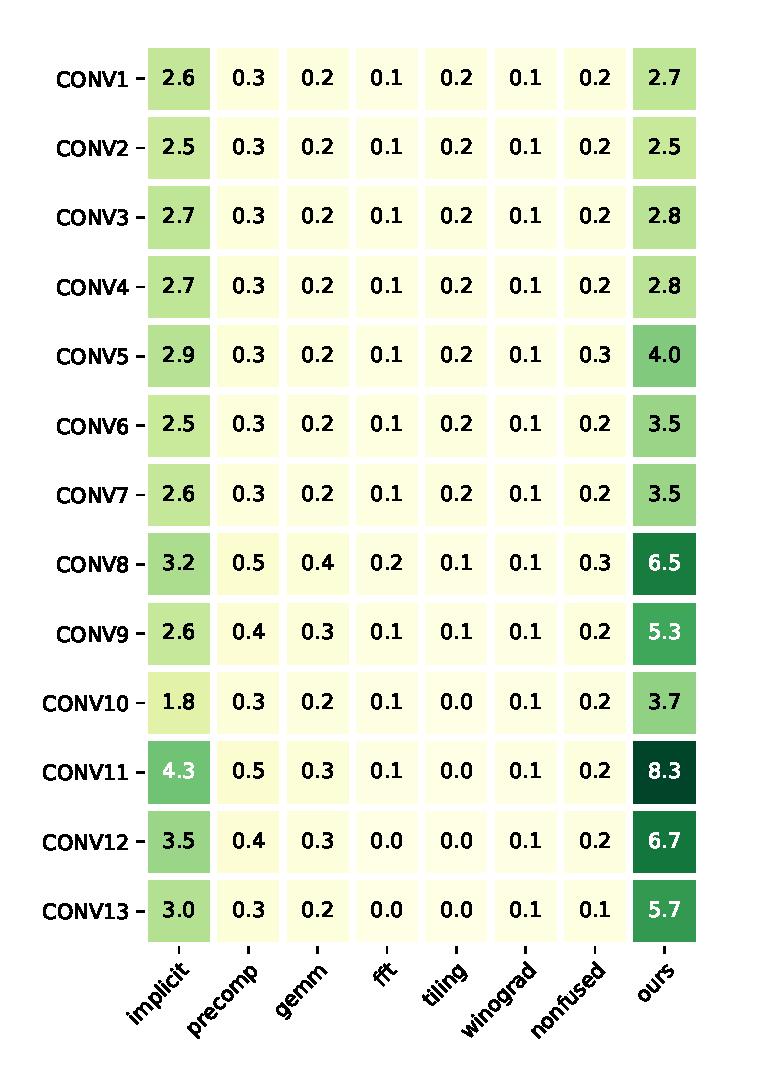
\includegraphics[width=\columnwidth,height=6.8cm]{./figure/depthwise_f3.eps}
	\label{fig:f33druntime2080}}
\subfloat[Speedups for the filter of size $5 \times 5$.]{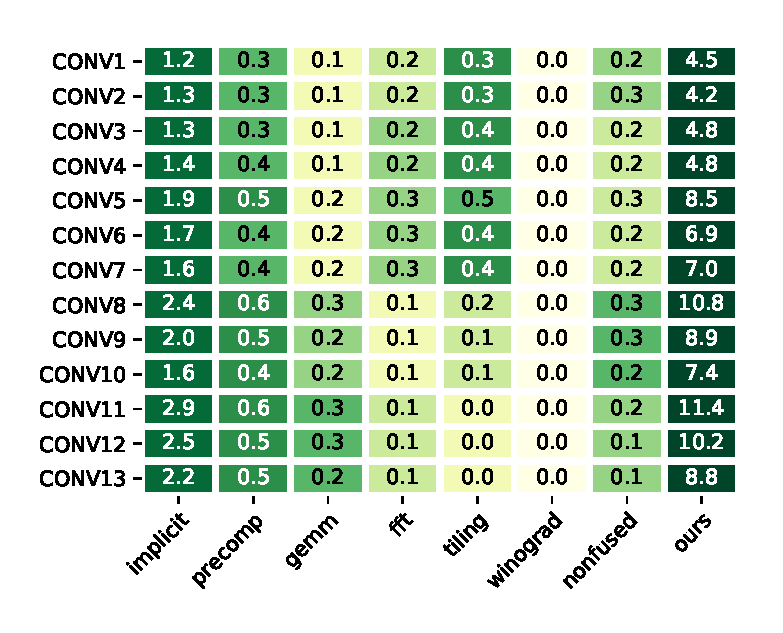
\includegraphics[width=\columnwidth,height=6.8cm]{./figure/depthwise_f5.eps}
	\label{fig:f53druntime2080}}

\caption{Speedups of our implementation and seven cuDNN algorithms over the baseline implementation for the depth-wise convolution.}
\label{fig:3druntime}
\end{figure*}


\subsubsection{Setup} In this experiment, we compare our approach against the depth-wise
convolution given by cuDNN. We compare to seven algorithms in cuDNN, including IMPLICIT\_GEMM (implicit), IMPLICIT\_PRECOMP\_GEMM
(precomp), GEMM (gemm), FFT (fft), FFT\_TILING (tiling), WINOGRAD (winograd) and WINOGRAD\_NONFUSED (nonfused). As Winograd is not
applicable  to a $5 \times 5$ filter, we do not report performance of Winograd when using a $5 \times 5$ filter. We use the convolutional
layer configurations that use depth-wise convolution from three popular embedded models, MobileNetv2, ShuffleNetv2 and EfficientNet. We
report the performance when the input and output batch sizes are set to 512, but we observe similar performance when using a different
batch size. Table \ref{tab:3dconvconfigs} gives he layer configurations used in this experiment.


%In the depth-wise convolution, one input element only needs to be convolved with
%one filter, while in the multi-channel 2D convolution, one input element needs to be convolved with all filters. Therefore, depth-wise
%convolutions require much less computation than multi-channel 2D convolutions, which makes depth-wise convolutions more sensitive to memory
%performance.


%Nowadays, depth-wise convolutions have been widely used in embedded CNNs, including MobileNetv2 \cite{Sandler_2018_CVPR}, EfficientNet
%\cite{tan2019efficientnet} and ShuffleNetv2 \cite{Ma_2018_ECCV}. In this section, we present the performance comparison of the depth-wise
%convolution between cuDNN and our implementation. We implement a simple depth-wise convolution and report speedups of cuDNN and our
%implementation over the simple depth-wise convolution. We evaluate 7 algorithms in cuDNN, including IMPLICIT\_GEMM (implicit),
%IMPLICIT\_PRECOMP\_GEMM (precomp), GEMM (gemm), FFT (fft), FFT\_TILING (tiling), WINOGRAD (winograd) and WINOGRAD\_NONFUSED (nonfused).
%Winograd can not be applied on a $5 \times 5$ filter, thus we set speedups for this algorithm to 0.

%We collect configurations of the convolutional layers using depth-wise convolution from three popular mobile embedded models,
%namely, MobileNetv2, ShuffleNetv2 and EfficientNet.
%Then, we set the number of the batch size to 512 ($I_N=O_N=512$). Other batch sizes demonstrate a similar performance because all tested implementations have a linear scale as the batch size. The exact configuration is presented in Table \ref{tab:3dconvconfigs}.

The speedups are shown in Figure \ref{fig:3druntime}. Our approach clearly performs best in all test cases. We obtain an average speedup of
$4.5\times$ and $7.6\times$ for the $3 \times 3$ and $5 \times 5$ filters, respectively. The implicit algorithm is the fastest algorithm in
cuDNN in all test cases. It achieves an average speedup of $2.8\times$ and $1.8\times$ for the $3 \times 3$ and $5 \times 5$ filters,
respectively. Compared with the fastest algorithm of cuDNN, the proposed approach achieves an average speedup of $1.5\times$, with the
maximum speedup reaching $2\times$ for the $3 \times 3$ filter, and an average speedup of $4\times$, with the maximum speedup reaching
$4.5\times$ for the $5 \times 5$ filter.

The algorithms of cuDNN except implicit algorithm perform poorly in all test cases and the speedups of these algorithms all below 1.
Considering that cuDNN is a closed source, we can only guess that FFT- and Winograd- based algorithms focus on reduction of computation and
trades memory performance for speed. Precomp and gemm algorithms need extra memory operations to compute output elements. Moreover,
depth-wise convolution is more sensitive to memory performance than multi-channel 2D convolution. Consequently, these algorithms perform
poorly on depth-wise convolutions.

\begin{figure}
\centering

\subfloat[Memory throughput for the filter of size $3 \times 3$.]{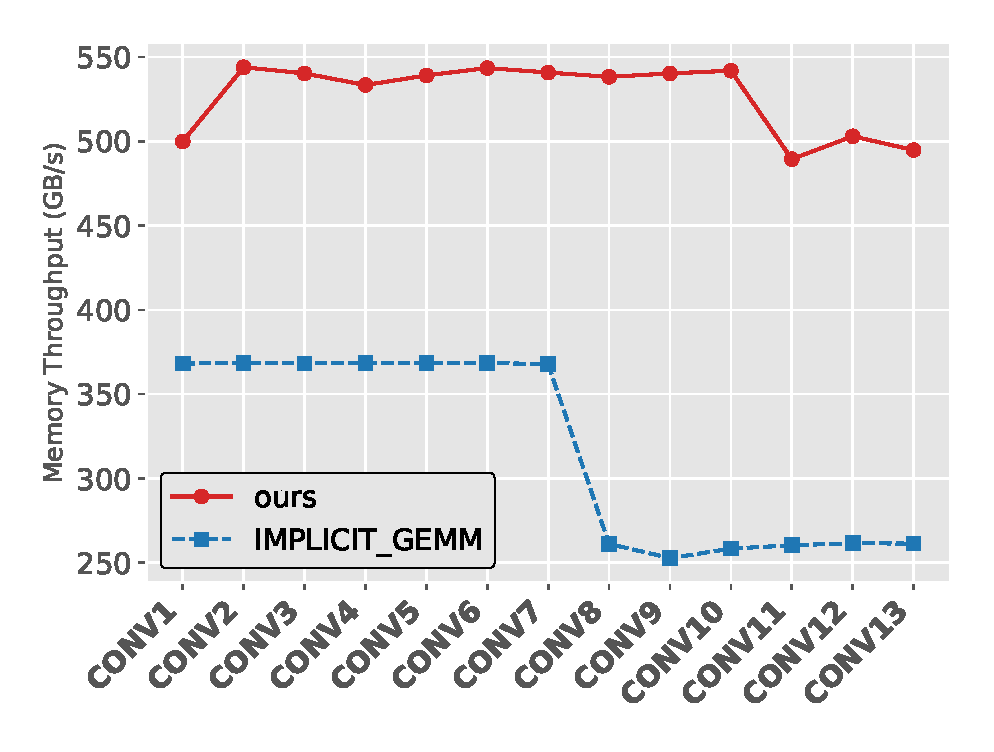
\includegraphics[width=\columnwidth,height=6cm]{./figure/depwisememthroughput.eps}
	\label{fig:depwisememthr}}
\hspace{0em}
\subfloat[Max bandwidth for the filter of size $3 \times 3$.]{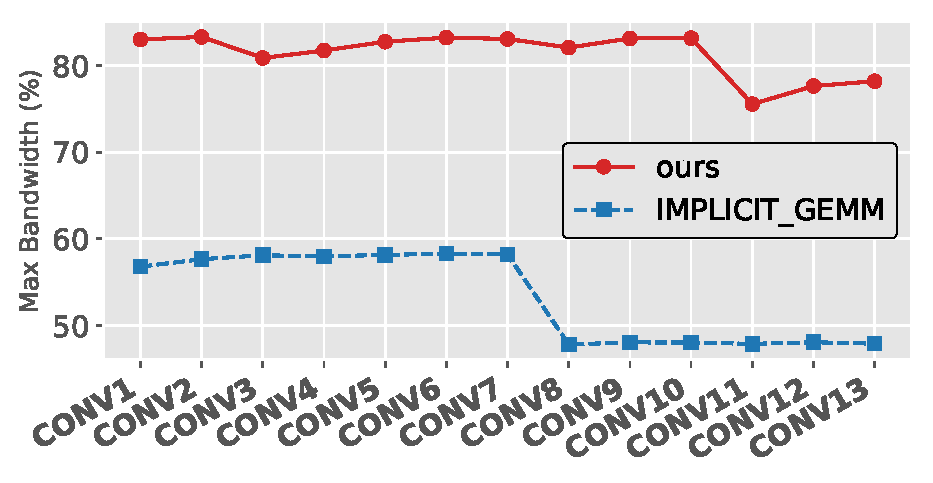
\includegraphics[width=\columnwidth,height=6cm]{./figure/depwisemembandwidth.eps}
	\label{fig:depwisemaxband}}
	
\caption{Memory analysis of cuDNN implicit algorithm and our implementation for the filter of size $3 \times 3$.}
\label{fig:depwisememanaly}
\end{figure}

Figure \ref{fig:depwisememanaly} demonstrates the memory throughput and max bandwidth for our implementation and cuDNN implicit algorithm when convolving with a $3 \times 3$ filter. We can see that our implementation achieves $1.5 \times$ memory throughput and max bandwidth compared with the implicit algorithm. This demonstrates that our reuse algorithms can improve the memory performance significantly.

In summary, both of reuse algorithms can significantly improve the memory throughput and max bandwidth, which leads to the performance improvements of depth-wise convolutions.  In contrast to the fastest algorithms in cuDNN, which is the state-of-the-art convolution library, our implementation achieves an average speedup of $1.5\times$ and $4\times$ for the $3 \times 3$ and $5 \times 5$ filters, respectively.

\subsection{Multi-channel 2D Convolution}
\label{multicconvexp}

\begin{table}[]
\caption{Configurations of multi-channel 2D convolution}
\label{tab:3dconvconfigs}
\begin{tabular}{c|ccccc}
\hline
& $I_N$ & $I_C=F_C$ & $I_H \times I_W$ & $F_N$ & $F_H \times F_W$ \\
\hline
CONV1 & 128  & 1,3       & $28\times 28$     & 128  & $3\times 3$       \\
CONV2 & 128  & 1,3       & $56\times 56$     & 64   & $3\times 3$       \\
CONV3 & 128  & 1,3       & $12\times 12$     & 64   & $5\times 5$       \\
CONV4 & 128  & 1,3       & $14\times 14$     & 16   & $5 \times 5$       \\
CONV5 & 128  & 1,3       & $24\times 24$    & 256  & $5 \times 5$       \\
CONV6 & 128  & 1,3       & $24\times 24$     & 64   & $5\times 5$       \\
CONV7 & 128  & 1,3       & $28\times 28$     & 16   & $5\times 5$       \\
CONV8 & 128  & 1,3       & $28\times 28$     & 512   & $3\times 3$       \\
CONV9 & 128  & 1,3       & $56\times 56$     & 256  & $3\times 3$       \\
CONV10 & 128  & 1,3       & $112\times 112$     & 128   & $3\times 3$       \\
CONV11 &128  & 1,3       & $224\times 224$     & 64   & $3\times 3$      \\
\hline
\end{tabular}
\end{table}

\begin{figure*}
\centering
	
\subfloat[Speedups for one input channel.]{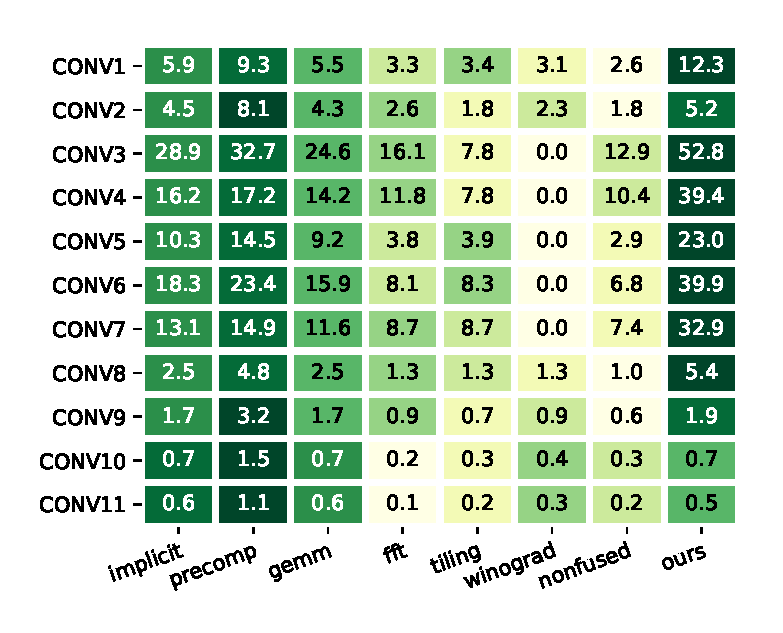
\includegraphics[width=\columnwidth,height=6.8cm]{./figure/multic2d_c1.eps}
	\label{fig:multic1runtime2080}}
\subfloat[Speedups for three input channels.]{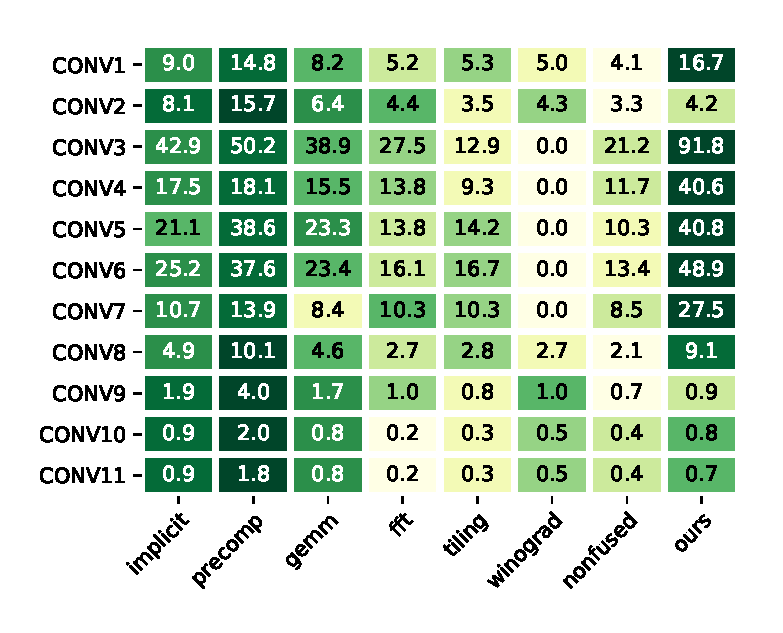
\includegraphics[width=\columnwidth,height=6.8cm]{./figure/multic2d_c3.eps}
	\label{fig:multic3runtime2080}}

\caption{Speedups of our implementation and cuDNN over im2col for one and three input channels.}
\label{fig:multi2druntime}
\end{figure*}


We apply Algorithm \ref{algo:basic}, \ref{algo:basic2} and \ref{algo:rowreuse} on multi-channel 2D convolutions with one and three input channels. The focus of this study is to optimize the memory transactions, and our implementation of multi-channel 2D convolutions do not optimize on input channels. Therefore, our implementation is suitable for convolutions with one and three input channels, which are normally the first layers of a CNN.

In this section, we present the performance comparison of the multi-channel 2D convolutions among three implementations, that is, cuDNN, im2col and our implementation. We collect the configurations of the convolutional layers using $3 \times 3$ and $5 \times 5$ filers from four popular CNN models,
namely, AlexNet \cite{Krizhevsky2012ImageNet}, VGG \cite{SimonyanZ14a}, ResNet \cite{HeZRS16} and GoogleLeNet \cite{SzegedyLJSRAEVR15}.
Then, we set the number of input channels to one and three ($I_C=F_C \in \{1, 3\}$) and the batch size to 128 ($I_N=O_N=128$). The exact configuration is presented in Table \ref{tab:3dconvconfigs}.

The speedups of our implementation and cuDNN over im2col are shown
in Figure \ref{fig:multi2druntime}. Our
implementation achieves average speedups of 19.5$\times$ and 25.6$\times$ relative to im2col for one and three input channels, respectively. Compared with the fastest algorithm in cuDNN, the proposed approach achieves an average speedup of 1.23$\times$ and 1.13$\times$ for one and three input channels, respectively.
%Different from depth-wise convolution, FFT- and Wingorad-based convolutions performs well for multi-channel 2D convolutions. The reason is that, multi-channel 2D convolution is computation intensive and reduction on computation can significantly improve the performance of multi-channel 2D convolution. Both FFT- and Winograd-based convolutions can reduce the computation and improve the performance of multi-channel 2D convolution.

In summary, our reuse algorithms can accelerate multi-channel 2D convolutions with small input channels.
